% \title{Busca Sequencial}
\title{Pesquisa Linear}
\maketitle

\begin{frame}{Busca Linear em memória principal}

  \begin{block}{Introdução}
    \small
    \begin{itemize}[<+-| alert@+>]
    \item O dados estarão sempre armazenados na \alert{memória principal}
      (DRAM\footnote{{\it Dynamic Random Access Memory\/} -- memória de
        acesso aleatório dinâmica}): não há necessidade de acesso à memória
      secundária (disco rígido, DVD, CD, {\it pendrive\/}, $\ldots$);
    \item O termo \alert{registro} é utilizado para armazenar a
      informação, sendo identificado a partir de uma \alert{chave} $k$;
    \item Dada uma chave $k$, esta chave deve ser única para no conjunto de \alert{registros};
    \item Os registros são armazenados em \alert{tabela} ou
      \alert{arquivo}, onde \alert{tabela} é usualmente usada para indicar
      um arquivo pequeno, e \alert{arquivo} é utilizado para indicar uma
      tabela grande;
    \item Um conjunto de arquivos é comumente chamado de \alert{banco de
        dados}.
    \end{itemize}
  \end{block}

\end{frame}

\begin{frame}{Busca Linear}

  \begin{block}{Aplicações}
    \begin{itemize}[<+-| alert@+>]
    \item Tabela de funções: Dada uma tabela da função $f(x)$ e dado um $x$, achar o valor
      da função $f$;
    \item Tradutor: dada uma palavra $w$ em português, buscar a(s)
      palavra(equivalente) em inglês.
    \end{itemize}
  \end{block}

\end{frame}  


\begin{frame}{Tipo abstrato de dados: Registro}

  \lstinputlisting[firstline=4,lastline=11]{../search/busca.h}

  \lstinputlisting[firstline=13,lastline=16]{../search/busca.h}

\end{frame}

% \begin{frame}{Busca sequencial simples: ideia}
%   animategraphics[step,scale=.75]{1}{img/searchS}{}{}
% \end{frame}

% \begin{frame}{Busca sequencial simples: algoritmo}

%   \begin{block}{Algoritmo S}

%     Dada uma tabela de registros $R_0, R_1, \ldots, R_{N-1}$, cujas
%     respectivas chaves são $k_0, k_1, \ldots, k_{N-1}$, este algoritmo
%     procura por um dado argumento $k$, assumindo $N\geq 1$.

%     \begin{description}[<+-| alert@+>]
%     \item[S1. [Inicializa.]] Atribui $i\leftarrow 0$.
%     \item[S2. [Compara.]] Se $k=k_i$, o algoritmo termina com sucesso.
%     \item[S3. [Avança]] Aumenta $i$ em $1$ unidade.
%     \item[S4. [Fim do arquivo?]] Se $i<N$, volte para S2. Caso contrário, o algoritmo
%       termina sem sucesso.
%     \end{description}
%   \end{block}

% \end{frame}

\begin{frame}{Busca sequencial simples: fluxograma}

  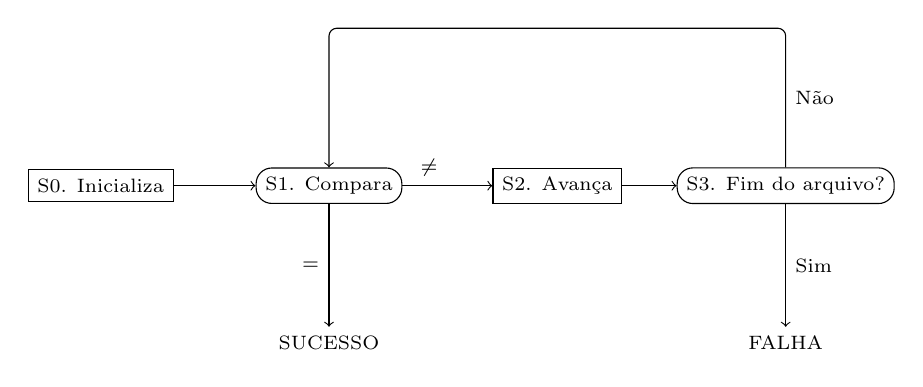
\begin{tikzpicture}

    \def\tikzshift{2cm}
    \tikzset{
      every node/.style={font=\scriptsize},
      every path/.style={draw},
      thestep/.style={draw},
      branch/.style={rounded corners=2mm,draw}
    }


    \def\X{\tikzshift}
    \def\thefactor{1.45}

    \foreach \x/\instr\sty in {0/{S0. Inicializa}/thestep, 1/{S1. Compara}/branch,
      2/{S2. Avança}/thestep, 3/{S3. Fim do arquivo?}/branch} {
      \node[\sty] (S\x) at (\thefactor*\x*\X,0) {\instr};
    }
    \node (SUCCESS) at (\thefactor*\X,-\X) {SUCESSO};
    \node (FAILURE) at (3*\thefactor*\X,-\X) {\alert{FALHA}};

    \path[->] (S0) -- (S1);
    \path[->] (S1) -- node[above left] {$\neq$} (S2);
    \path[->] (S2) -- (S3);
    \path[->,rounded corners=1mm] (S3) -- node [right]{Não} +(0,\tikzshift) -| (S1);

    \path[->] (S1) -- node[left] {$=$} (SUCCESS);
    \path[->] (S3) -- node[right] {Sim} (FAILURE);
  \end{tikzpicture}

\end{frame}

\begin{frame}{Busca sequencial simples: programa}


  \lstinputlisting[firstline=5,lastline=17]{../search/sequencial.c}

\end{frame}

\begin{frame}{Busca sequencial simples: desempenho}

  \begin{itemize}
  \item Melhor caso: $C_N=1$, a chave está na primeira posição da tabela;
  \item Pior caso: $C_N=N$, a chave não se encontra na tabela;
  \item Média: $\overline{C}_N=\frac{1+2+\ldots+N}{N}=\frac{N+1}{2}$
  \end{itemize}

  \noindent onde $C_N$ -- é o número de comparações em um conjunto
  (tabela) com $N$ elementos.

\end{frame}

% \begin{frame}{Busca sequencial rápida: ideia}
%   animategraphics[step,scale=.75]{1}{img/searchQ}{}{}
% \end{frame}


% \begin{frame}{Busca sequencial rápida: algoritmo}


%   \begin{block}{Algoritmo Q}

%     É parecido com o Algoritmo S, exceto que ele assume a existência de um
%     registro fictício $R_N$ no final do arquivo, contendo a chave
%     buscada. Com este artifício dentro do loop {\tt for} compara-se a
%     chave procurada com a $i-$ésima chave. Ao término do loop, se o índice
%     $i$ for igual a $N$, significa que a chave não se encontra no arquivo.

%     \begin{description}[<+-| alert@+>]
%     \item[Q0. [Inicializa.]] Atribui $i\leftarrow 0$ e $k_N\leftarrow k$.
%     \item[Q1. [Compara.]] Se $k=k_i$, vá para Q4.
%     \item[Q2. [Avança]] Aumente $i$ em $1$ unidade.
%     \item[Q3. [Fim do arquivo?]] Se $i<N$, o algoritmo termina com sucesso. Caso contrário, o algoritmo
%       termina com falha ($i=N$).
%     \end{description}
%   \end{block}

% \end{frame}

% \begin{frame}{Busca sequencial rápida: programa}


%   \lstinputlisting[firstline=19, lastline=40]{sequencial.c}

% \end{frame}

% \begin{frame}{Busca sequencial em tabela ordenada: ideia}
%   animategraphics[step,scale=.75]{1}{img/searchT}{}{}
% \end{frame}

% \begin{frame}{Busca sequencial em tabela ordenada: algoritmo}

%   Dada uma tabela de registros $R_0, R_1, \ldots, R_{N-1}$ cujas chaves
%   estão em ordem crescente $k_0, k_1, \ldots, k_{N-1}$, este algoritmo
%   procura por um dado argumento $k$. O algoritmo assume que há um
%   registro fictício $R_N$ cujo valor da chave é $k_{N}=\infty > k$.

%   \begin{description}
%   \item[T0. [Inicializa.]] Atribui $i\leftarrow 0$ e $k_N=\infty$.
%   \item[T1. [Compara.]] Se $k\geq k_i$, vá para T3.
%   \item[T2. [Avança]] Aumente $i$ em $1$ unidade e retorne para T1.
%   \item[T3. [Igualdade?]] Se $k=k_i$, o algoritmo termina com sucesso. Caso contrário, o algoritmo
%     termina com falha.
%   \end{description}

% \end{frame}

% \begin{frame}{Busca sequencial em tabela ordenada: programa}
%   \lstinputlisting[basicstyle=\scriptsize,firstline=41,lastline=53]{sequencial.c}
% \end{frame}
